\zag{Введение}
\thispagestyle{empty}
\subzag{Предмет и метод молекулярной оптики}

Молекулярная оптика есть часть физики, посвященная изучению
процессов взаимодействия электромагнитного излучения с веществом,
процессов, определяемых микроскопической структурой вещества и
молекулярной динамикой газов, жидкостей, растворов,
кристаллов и жидких кристаллов.

Эта самостоятельная область знаний характеризуется единым методом
исследования большого многообразия явлений, которые удалось
истолковать в рамках электронной теории, учитывающей строение,
электрические и оптические свойства атомов и молекул. Задача этой
области науки заключается в том, чтобы выразить свойства среды
через молекулярные константы. Обратная задача исходит из
утверждения возможности установить однозначную связь между
свойствами молекул и свойствами среды. Это возможно, если
молекулы сохраняют в среде свою индивидуальность (слабое
межмолекулярное взаимодействие). Молекулярная оптика изучает
следующий ряд явлений, связанных с важнейшей характеристикой
молекулы --- ее поляризуемостью: преломление, отражение и
поглощение света изотропными и анизотропными средами;
дисперсия света; рассеяние света; естественная оптическая
активность молекул; вынужденное двойное лучепреломление в силовых
полях (в электрическом~--- явление Керра, в магнитном~--- явление
Коттон-Мутона, в поле градиента скорости~--- явление Максвелла). В
молекулярной оптике устанавливается связь между этими явлениями.
Все они в той или иной мере определяются тензором 2-го ранга~---
поляризуемостью молекулы.

В настоящее время мы имеем возможность вводимые в молекулярную
оптику феноменологические константы (составляющие тензора
поляризуемости) выразить через величины, непосредственно
характеризующие строение электронной оболочки молекулы. Такими
величинами являются характеристики энергетических уровней и
вероятности перехода между ними.

В конечном счете, ключ к раскрытию сущности оптических свойств
молекулы дают частоты и интенсивности в ее спектре, поэтому в
основе молекулярной оптики лежит молекулярная спектроскопия.
Физические величины, характеризующие свойства микроскопических
объектов~--- атомов и молекул,~--- могут быть определены
теоретически только при помощи квантовой механики.
Квантово-механическая теория явлений молекулярной оптики, в
частности явления дисперсии света, хорошо разработана и приводит
к таким же результатам, что и классическая теория. Это позволяет
пользоваться классической полуэмпирической теорией
молекулярно-оптических явлений, дающей не только качественное, но
и количественное их объяснение и вскрывающей их внутренние
связи. Эта теория основывается, с одной стороны, на общих
положениях электромагнитной теории света и свойствах
излучающего электрона, с другой~--- на химической теории строения
молекул.

Таким образом, молекулярно-оптическими называются такие явления,
в которых находят свое отражение не только свойства света, но и
свойства среды, с которой он взаимодействует. Тем самым, явления
молекулярной оптики представляют один из наиболее важных
источников информации о строении и свойствах молекул, жидкостей,
кристаллов, высокомолекулярных веществ и коллоидных систем. Этим
определяется большое прикладное значение молекулярной оптики, ее
применение в технике, в различных областях физики, химии,
метеорологии, астрономии.

\subzag{Основные законы электромагнитной теории света}
Далее предполагается, что читатель уже знаком с
основами теории электромагнитного поля. Поэтому приводятся лишь
основные положения электромагнитной теории света.

Электромагнитная волна в вакууме характеризуется значениями
векторов напряженности электрического поля $\vec E$ и магнитного
поля $\vec H$. В веществе электромагнитное поле световой волны
характеризуется векторами электрической и магнитной индукции $\vec
D$ и $\vec B$, векторами $\vec E$ и $\vec H$, плотностью
электрических зарядов $\rho$, а также (в случае проводников)
плотностью тока проводимости $\vec j$. Свойства электромагнитного
поля передаются уравнениями Максвелла:
\begin{plain}$$\eqalign{\rot\vec H=& {1\over c}{\partial\vec D\over\partial t}
+{4\pi\over c}\vec j,\cr \rot\vec E=& -{1\over c}{\partial\vec
B\over\partial t},\cr \diverg\vec D=& 4\pi\rho,\cr \diverg\vec
B=& 0.}\noq$$\end{plain} Здесь $c$ --- скорость света в вакууме
($3\cdot10^{10}\ {\rm \hbox{см}\cdot \hbox{сек}^{-1}}$). Связь между \hbox{пятью}
векторами поля дается соотношениями (справедливыми для изотропной
среды):
\begin{plain}$$\eqalign{\vec j=&\sigma\vec E,\cr
\vec D=&\varepsilon\vec E,\cr \vec B=&\mu\vec H.}\noq$$\end{plain} Здесь
$\sigma$ --- удельная электропроводность, $\varepsilon$ --- диэлектрическая
постоянная и $\mu$ --- магнитная проницаемость вещества. Величины
$\varepsilon$ и $\mu$ безразмерны, электропроводность имеет
размерность ${\rm \hbox{сек}^{-1}}$. В общем случае анизотропного тела
электропроводность, диэлектрическая постоянная и магнитная
восприимчивость анизотропны и выражаются тензорами. Рассматриваем,
главным образом, взаимодействие со светом немагнитных
диэлектриков, для которых $\sigma=0$ и $\mu=0$. Связь между
индукцией и напряженностью может быть выражена и иначе,
посредством вектора поляризации вещества (электрической или
магнитной). Имеем в электрическом поле:
$$\vec D=\varepsilon\vec E=\vec E+4\pi\vec P,\noq$$
или
$$\vec P={\varepsilon-1\over4\pi}\vec E.\noq$$
Вектор $\vec P$ характеризует электрический дипольный момент
единицы объема вещества. Объемная плотность энергии
электромагнитного поля равна:
$$W={1\over8\pi}\vec E\vec D+{1\over8\pi}\vec H\vec B.\noq$$
Напряженности поля могут быть выражены через потенциалы поля.
Ввиду вихревого характера магнитного поля можно положить:
$$\vec B=\rot\vec A,\noq$$
где $\vec A$ --- вектор-потенциал поля. Подставляя это уравнение
во второе уравнение \eqn{1}, получаем:
$$\rot\left(\vec E+{1\over c}{\partial\vec A\over\partial
t}\right)=0.\noq$$ Уравнение \eqn{7} удовлетворяется выражением:
$$\vec E=-{1\over c}{\partial\vec A\over\partial
t}-\grad\varphi.\noq$$ Так как ротор от градиента скаляра
тождественно равен нулю: $\rot\,\grad\varphi\equiv0$, то $\varphi$
--- скалярный потенциал поля.
\par\noindent Уравнение \eqn{6} определяет ротор вектор-потенциала. Задав
дивергенцию в виде
$$\diverg\vec A=-{\varepsilon\mu\over c}{\partial\varphi\over\partial
t},\noq$$ получаем из уравнений Максвелла уравнения для
потенциалов:
\begin{plain}$$\eqalign{\nabla^2\vec A-{\varepsilon\mu\over
c^2}{\partial^2\vec A\over\partial t^2}=&\hbox{\ }-{4\pi\mu\over c}\vec
j,\cr \nabla^2\varphi-{\varepsilon\mu\over
c^2}{\partial^2\varphi\over\partial t^2}=&\hbox{\ }-{4\pi\over\varepsilon}
\rho.}\noq$$\end{plain} В отсутствие свободных зарядов и токов оба потенциала
удовлетворяют волновому уравнению:
$$c'={c\over\sqrt{\varepsilon\mu}},\hskip 5mm\nabla^2\Psi={1\over
{c'}^2}{\partial^2\Psi\over\partial t^2}.\noq$$
Сферически-симметричное решение волнового уравнения описывает
сферическую электромагнитную волну:
$$\Psi={1\over R}\left\{f_1\left(t-{R\over c'}\right)+f_2
\left(t+{R\over c'}\right)\right\},\noq$$ где $f_1,\ f_2$ ---
произвольные функции. Первый член \eqn{12} представляет
сферическую волну, исходящую из некоторого источника поля и
распространяющуюся со скоростью $c'$; второй --- волну, приходящую
из бесконечности и сходящуюся в истоке поля. Нас будет
интересовать только первая часть решения \eqn{12}:
$$\Psi={1\over R}f\left(t-{R\over c'}\right).\eqno (1.12\hbox{\it a})$$
Источниками переменного электромагнитного поля служат движущиеся
заряды. Решение \eqn{12{\it a}} в явной форме имеет вид:
\begin{plain}$$\eqalign{\varphi=&{1\over R}\int{\rho\left(t-{R\over
c'}\right)\over R}dV\cr \vec A=&{\mu\over c}\int{\vec
j\left(t-{R\over c'}\right)\over R}dV.}\noq$$\end{plain} Интегрирование
проводится по всему объему. Для нахождения поля в некоторой точке
в момент $t$ нужно для каждого элемента объема $dV$ определить тот
заряд и ток, которые находились в $dV$ в момент $\left(t-{R\over
c'}\right)$, где $R$ --- расстояние от $dV$ до точки, в которой
определяется поле.

Потенциалы \eqn{13} --- запаздывающие потенциалы. Сферическая
волна уносит из излучающего объема определенное количество
энергии. Если потеря энергии происходит только посредством
излучения, то мы можем написать:
$$-{\partial W\over\partial t}={\partial\over\partial
t}\int{\omega dV}=-{1\over8\pi}{\partial\over\partial t}\int(\vec
E\vec D+\vec H\vec B)dV=\int\limits_{S}S_ndS,\noq$$ где $S_n$ ---
проекция вектора потока энергии на нормаль к элементу поверхности
$dS$, охватывающий излучающий объем. Вектор потока энергии
называется вектором Умова---Пойнтинга:
$$\vec S={c\over4\pi}[\vec E\vec H].\noq$$
Для того, чтобы получить непосредственные выражения $\vec E$ и
$\vec H$ сферической электромагнитной волны, необходимо, очевидно,
задаться определенной характеристикой излучателя. Однако, так или
иначе, ясно, что на достаточно большом удалении от излучателя
ограниченный участок сферической волны может считаться плоским.
Следовательно, если $z$ есть направление нормали к этому участку
--- направление распространения волны, имеем:
$$\vec E=\vec E(z,t);\hskip 4mm\vec H=\vec H(z,t)\noq$$
и, считая волну монохроматической, т.е. зависящей от времени по
гармоническому закону, получаем:
$$\vec E=\vec E(z)e^{iwt};\hskip 4mm \vec H=\vec
H(z)e^{iwt}.\eqno (1.16\hbox{\it a})$$ Рассмотрим плоскую волну в однородном
диэлектрике, лишенном свободных зарядов. Из \eqn{1} и \eqn{2}
имеем:
$${\varepsilon\over c}{\partial\vec E\over\partial t}=\rot\vec
H.$$ Дифференцируя это уравнение по времени и подставляя в него
значение ${\partial\vec H\over\partial t}$ из второго уравнения
\eqn{1}, получаем в конце концов:
$${\varepsilon\mu\over c^2}{\partial^2\vec E\over\partial
t^2}=\nabla^2\vec E,\noq$$ и аналогично:
$${\varepsilon\mu\over c^2}{\partial^2\vec Н\over\partial
t^2}=\nabla^2\vec H.\eqno (1.17\hbox{\it a})$$ Подставляя \eqn{16{\it a}} в
\eqn{17} и \eqn{17{\it a}}, находим:
\begin{plain}$$\eqalign{\vec E=&\vec E_{01}e^{i(wt-kz)}+\vec
E_{02}e^{i(wt+kz)},\cr \vec H=&\vec H_{01}e^{i(wt-kz)}+\vec
H_{02}e^{i(wt+kz)}}.\noq$$\end{plain} Здесь $k=w{\sqrt{\varepsilon\mu}\over
c}={w\over c'}={2\pi\nu\over c'}={2\pi\over
c'T}={2\pi\over\lambda}$, $T$
--- период, $\lambda$ --- длина волны в среде, связанная с длиной
волны в вакууме $\lambda_0$ соотношением:
$$\lambda={c'\over c}\lambda_0.\noq$$
Первые члены \eqn{18} описывают плоскую электромагнитную волну,
распространяющуюся вдоль положительного, вторые --- волну,
распространяющуюся вдоль отрицательного направления $z$.
Ограничимся рассмотрением первых членов. В общем случае можем
написать:
$$\vec E=\vec E_0e^{iw(t-{\vec r\vec s\over c'})}=\vec
E_0e^{i(wt-\vec k\vec r)},\noq$$ и аналогично для $\vec H$. Здесь
$\vec s$ --- единичный вектор нормали к волне, $\vec k$ ---
волновой вектор:
$$\vec k={2\pi\vec s\over \lambda}.$$
Подставляя \eqn{20} в уравнения Максвелла, после несложных
преобразований находим:
$$\vec E\vec s=0,\hskip 4mm\vec H\vec s=0, \hskip 4mm\vec E\vec
H=0.\noq$$ Эти уравнения выражают поперечность световой волны и
взаимную перпендикулярность $\vec E$ и $\vec H$.

Световая волна может характеризоваться различными состояниями
поляризации. У естественного света плоскости, в которых колеблются
перпендикулярные друг другу векторы $\vec E$ и $\vec H$, не
фиксированы, и между составляющими этих векторов нет определенных
соотношений вследствие хаотического разброса поляризаций отдельных
волновых цугов. В усреднении по времени:
$$\overline{E_x^2}=\overline{E_y^2}=\overline{E_z^2},\hskip 4mm
\overline{E_xE_y}=\overline{E_yE_z}=\overline{E_zE_x}=0,$$ и
аналогично для $H$.

Плоско(линейно)-поляризованная волна характеризуется определенным
направлением колебаний векторов $\vec E$ и $\vec H$. При этом
плоскостью поляризации световой волны принято называть плоскость,
в которой колеблется магнитный вектор, иными словами, плоскость,
перпендикулярную к плоскости колебаний электрического вектора.
Если отдельные составляющие волны \eqn{20} характеризуются
различными значениями фазы, волна в общем случае является
эллиптически поляризованной.

Пусть $s=s_z$ и (в вещественной форме)
\begin{plain}$$\eqalign{E_x=&A_1\cos(\tau+\delta_1)\cr
E_y=&A_2\cos(\tau+\delta_2).}$$\end{plain} Здесь $\tau=w\left(t-{\vec r\vec
s\over c'}\right)$. Исключая $\tau$, находим:
$$\left({E_x\over A_1}\right)^2+\left({E_y\over
A_2}\right)^2-2{E_x\over A_1}{E_y\over
A_2}\cos(\delta_2-\delta_1)=\sin^2(\delta_2-\delta_1).\noq$$ Это
уравнение является уравнением эллипса. В частном случае, при
$\delta_2-\delta_1=$\linebreak$=2n{\pi\over2}$ имеем линейную поляризацию, а в
случае $A_1=A_2$ и $\delta_2-\delta_1=$\linebreak$=(2n+1){\pi\over2}$~---
круговую ($n=0,\pm1,\pm2,...$). Если
$\delta_2-\delta_1={\pi\over2}+2|n|\pi$,~ т.~е.
\begin{plain}$$\eqalign{E_x=&A\cos(\tau+\delta_1),\cr
E_y=&-A\sin(\tau+\delta_1),}$$\end{plain}волна~--- правая, а если
$\delta_2-\delta_1=-{\pi\over2}+2|n|\pi$, т.~е.
\begin{plain}$$\eqalign{E_x=&A\cos(\tau+\delta_1),\cr
E_y=&A\sin(\tau+\delta_1),}$$\end{plain}волна~--- левая. Если смотреть
навстречу распространяющейся волне, то в первой волне
электрический вектор обходит окружность по направлению часовой
стрелки. В комплексной форме эллиптически поляризованная волна
характеризуется соотношением вида
$${E_y\over E_x}=a+bi,$$
причем, для линейно поляризованной волны $b=0$. В случае правой и
левой круговой волны соответственно:
$${E_y\over E_x}=i,\hskip 4mm{E_y\over E_x}=-i.$$
Нетрудно установить соотношение между $a$ и $b$, с одной стороны,
и $A_1,\ A_2$ и $(\delta_2-\delta_1)$ --- с другой.

К этому мы вернемся далее.\pagebreak

\subzag{Тензор поляризуемости} 
\shortpage
Оптические свойства
среды (немагнитного диэлектрика) характеризуются в общем
анизотропном случае тензором диэлектрической постоянной для
электромагнитных волн. В изотропной среде, согласно
электромагнитной теории света, диэлектрическая постоянная связана
с показателем преломления соотношением:
$$\varepsilon=n^2.$$
Согласно \eqn{3},
$$\varepsilon\vec E=\vec E+4\pi\vec P.$$
Вектор поляризации $\vec P$ выражает дипольный момент единицы
объема среды, в которой имеется поле $\vec E$. Если $N_1$ ---
число молекул в единице объема, то
$$\vec P=N_1\vec p_{\varepsilon},$$
где $\vec p_{\varepsilon}$ --- дипольный момент молекулы в
направлении поля. В быстропеременном электрическом поле световой
волны $\vec p_{\varepsilon}$ возникает лишь вследствие индукции
зарядов, но не благодаря ориентации полем дипольных молекул, так
как при больших частотах изменения поля молекулы не успевают
ориентироваться (дисперсия).

Индуцированный электрическим полем дипольный момент пропорционален
напряженности поля:
$$\vec p_{\varepsilon}=\alpha\vec E,\noq$$
$$\vec P=N_1\alpha\vec E.\eqno (1.23\hbox{\it a})$$
Коэффициент $\alpha$ выражает индукционную, электронную
поляризуемость молекулы --- способность ее электронов смещаться
под действием поля $\vec E$. Из~соотношения \eqn{23} следует
написать соотношения:
$$p_i=\sum\limits_{k}\alpha_{ik}E_k,\hskip 4mm i,k=x,y,z.\noq$$
Коэффициенты $\alpha_{ik}$ являются, тем самым, составляющими
тензора второго ранга. Тензор $\alpha_{ik}$ может быть
комплексным, что означает, очевидно, несовпадение фазы дипольного
момента $p_i$ с фазой действующей напряженности поля $E_k$. Такое
несовпадение может определяться, в частности, наличием вызванного
теми или иными причинами затухания колебаний электронов. В~этом
случае в молекуле действуют неконсервативные силы и некоторая
часть энергии электромагнитного поля поглощается --- имеет место
поглощение света. Исследуя вещество в спектральной области,
достаточно удаленной от собственных полос поглощения, можем
отвлечься от действия этих сил. В~отсутствии поглощения света
рассматриваемая система является консервативной, и тензор
поляризуемости $\alpha_{ik}$ должен быть эрмитовым, т.~е. должно
соблюдаться условие:
$$\alpha_{ik}=\alpha_{ki}^*.\noq$$
Следовательно, диагональные составляющие тензора $\alpha_{ii}$
обязательно вещественны.

Докажем, что консервативной системе должен соответствовать эрмитов
тензор поляризуемости.

Общее выражение для энергии поляризующейся молекулы в
электрическом поле имеет вид:
$$U={1\over2}\vec p\vec
E^*={1\over2}\sum\limits_{i,k}\alpha_{ik}E_i^*E_k.\noq$$ Это
выражение вещественно, каким и должно быть выражение для энергии.
Коэффициент ${1\over2}$ возникает при интегрировании:
$$U(x)=\int\limits_{0}^{E_x}p_xdE_x=\int\limits_{0}^{E_x}
\sum\limits_{k}\alpha_{xk} E_xdE_x={1\over2}p_xE_x.$$ Очевидно,
что
$$U^*=U={1\over2}\sum\limits_{i,k}\alpha_{ik}^*E_iE_k^*={1\over2}\sum
\limits_{i,k}\alpha_{ik}E_i^*E_k.$$ И, так как сумма не меняется
от перестановки индексов $i,k$:
$$U={1\over2}\sum\limits_{i,k}\alpha_{ik}E^*_iE_k={1\over2}\sum_{i,k}\alpha^*_{ki}
E^*_iE_k.$$ Условия \eqn{25} достаточно, чтобы удовлетворить этому
соотношению. Докажем, что оно необходимо.

Пусть на молекулу действует сила поля $E_x^*$, возрастающая от 0
до $E_x^*$. Работа, производимая этой силой, есть вещественная
величина, равная
$$A_{1x}=\int\limits_{0}^{E_x^*}p_xdE_x^*=\int\limits_{0}^{E_x^*}\alpha_{xx}E_xdE_x^*=
{1\over2}\alpha_{xx}|E_x|^2.$$ Подействуем теперь силой $E_y^*$,
возрастающей от 0 до $E_y^*$. Получим работу:
$$A_{1y}=\int\limits_{0}^{E_{y}^*}p_ydE_y^*=\int\limits_{0}^{E_y^*}(\alpha_{yx}
E_x+\alpha_{yy}E_y)dE_y^*=\alpha_{yx}E_xE_y^*+{1\over2}a_{yy}|E_y|^2.$$
Общая работа равна:
$$A_1=A_{1x}+A_{1y}={1\over2}\alpha_{xx}|E_x|^2+\alpha_{yx}E_xE_y^*+{1\over2}
\alpha_{yy}|E_y|^2.$$ Проведем теперь тот же процесс в обратном
порядке:
$$A_{2y}=\int\limits_{0}^{E_y^*}p_ydE_y^*=\int\limits_0^{E_y^*}\alpha_{yy}E_ydE^*_y=
{1\over2}\alpha_{yy}|E_y|^2,$$
$$A_{2x}=\int\limits_0^{E_x^*}p_xdE_x^*=\int\limits_0^{E_x^*}(\alpha_{xy}E_y+
\alpha_{xx}E_x)dE_x^*=\alpha_{xy}E_yE_x^*+{1\over2}\alpha_{xx}|E_x|^2,$$
$$A_2=A_{2y}+A_{2x}={1\over2}\alpha_{yy}|E_y|^2+\alpha_{xy}E_x^*E_y+{1\over2}\alpha_{xx}|E_x|^2.$$
Для консервативной системы вещественные величины $A_1=A_2$, и,
следовательно, $\alpha_{yx}=\alpha_{xy}^*$. Аналогичным образом
находим
$$\alpha_{zx}=\alpha_{xz}^*,\hskip 4mm\alpha_{zy}=\alpha_{yz}^*,$$
что и требовалось доказать.

Вещественная часть тензора поляризуемости, в силу его эрмитовости,
есть его симметричная часть:
$$S_{ik}={1\over2}\left(\matrix{
\alpha_{xx}&\alpha_{xy}&\alpha_{xz}\cr
\alpha_{yx}&\alpha_{yy}&\alpha_{yz}\cr
\alpha_{zx}&\alpha_{zy}&\alpha_{zz}\cr
}\right)+{1\over2}\left(\matrix{
\alpha_{xx}&\alpha_{xy}^*&\alpha_{xz}^*\cr
\alpha_{yx}^*&\alpha_{yy}&\alpha_{yz}^*\cr
\alpha_{zx}^*&\alpha_{zy}^*&\alpha_{zz}\cr }\right)=$$ $$=\left(\matrix{
\alpha_{xx}&{\alpha_{xy}+\alpha_{xy}^*\over2}&\alpha_{xz}^*\cr
{\alpha_{yx}+\alpha_{yx}^*\over2}&\alpha_{yy}&{\alpha_{yz}+\alpha_{yz}^*\over2}\cr
{\alpha_{zx}+\alpha_{zx}^*\over2}&{\alpha_{zy}+\alpha_{zy}^*\over2}&\alpha_{zz}\cr
}\right).$$ Действительно, согласно \eqn{25}, этот тензор
симметричен и равен:
$$\left(\matrix{
\alpha_{xx}&\alpha'_{xy}&\alpha'_{xz}\cr
\alpha'_{yx}&\alpha_{yy}&\alpha'_{yz}\cr
\alpha'_{zx}&\alpha'_{zy}&\alpha_{zz}\cr }\right),\noq$$ где
$$\alpha'_{xy}={1\over2}(\alpha_{xy}+\alpha_{xy}^*)=
{1\over2}(\alpha_{yx}+\alpha_{yx}^*)={1\over2}(\alpha_{xy}+\alpha_{yx})$$
являются вещественными величинами.

Напротив, мнимая часть эрмитова тензора антисиметрична:
$$A_{ik}={1\over2}\left(\matrix{
\alpha_{xx}&\alpha_{xy}&\alpha_{xz}\cr
\alpha_{yx}&\alpha_{yy}&\alpha_{yz}\cr
\alpha_{zx}&\alpha_{zy}&\alpha_{zz}\cr
}\right)-{1\over2}\left(\matrix{
\alpha_{xx}&\alpha_{xy}^*&\alpha_{xz}^*\cr
\alpha_{yx}^*&\alpha_{yy}&\alpha_{yz}^*\cr
\alpha_{zx}^*&\alpha_{zy}^*&\alpha_{zz}\cr
}\right)=$$$$=\left(\matrix{
0&{\alpha_{xy}-\alpha_{xy}^*\over2}&{\alpha_{xz}-\alpha_{xz}^*\over2}\cr
{\alpha_{yx}-\alpha_{yx}^*\over2}&0&{\alpha_{yz}-\alpha_{yz}^*\over2}\cr
{\alpha_{zx}-\alpha_{zx}^*\over2}&{\alpha_{zy}-\alpha_{zy}^*\over2}&0\cr
}\right)=\left(\matrix{ 0&\alpha''_{xy}&\alpha''_{xz}\cr
-\alpha''_{yx}&0&\alpha''_{yz}\cr
-\alpha''_{zx}&-\alpha''_{zy}&0\cr }\right).\noq$$ Здесь
$\alpha''_{xy}={1\over2}(\alpha_{xy}-\alpha_{xy}^*)={1\over
2}(\alpha_{xy}-\alpha_{yx})=-\alpha''_{yx}$ --- чисто мнимые
величины. Составляющие тензора второго ранга при преобразовании
координат преобразуются как произведение двух векторов. Очевидно,
что выражение $\alpha_{xy}-\alpha_{yx}$ преобразуется как $z$-овая
составляющая векторного произведения или аксиального вектора
$${1\over2}(\alpha_{xy}-\alpha_{yx})=i[\vec b\vec c]_z=id_z,$$
и антисиметричная часть эрмитова тензора приводится к виду
$$A_{ik}=i\left(\matrix{
0&d_z&-d_y\cr -d_z&0&d_x\cr d_y&-d_x&0\cr }\right).\eqno (1.28\hbox{\it a})$$
Следовательно, $\alpha_{ik}=S_{ik}+A_{ik}$, или
\begin{plain}$$\eqalign{\alpha_{xy}=&S_{xy}+i[\vec b\vec c]_z=S_{xy}+id_z,\cr
\alpha_{yx}=&S_{xy}-i[\vec b\vec c]_z=S_{xy}-id_z}$$\end{plain} и т.~д.

Во всех задачах молекулярной оптики, за исключением относящихся к
магнитному и естественному вращению плоскости поляризации света,
мы будем, в отсутствии поглощения света, иметь дело с вещественным
и, следовательно, симметричным тензором $S_{ik}$, для которого
сохраним обозначение $\alpha_{ik}$. Такому тензору соответствует
вещественный эллипсоид поляризуемости
$$\sum\limits_{x',y'}\alpha'_{x'y'}x'y'={\rm const}.\noq$$
Соответствующим поворотом осей координат этот эллипсоид может быть
преобразован к главным осям:
$$\sum\limits_x \alpha_{xx}x^2={\rm const}.\noq$$
Иными словами, тензор преобразуется к диагональной форме:
$$S_{ik}=i\left(\matrix{
\alpha_{xx}&0&0\cr 0&\alpha_{yy}&0\cr 0&0&\alpha_{zz}\cr
}\right).\eqno (1.27\hbox{\it a})$$ Напомним, каким образом осуществляется
это преобразование. Нужно найти направления главных осей
координат, в которых тензор принимает форму \eqn{27{\it a}}.
Следовательно, задача сводится к нахождению трех взаимно
ортогональных векторов, которые при умножении на тензор
\eqn{27{\it a}} не меняли бы своего направления, а изменялись бы
только по величине. При умножении на $S_{ik}$ произвольного
вектора, очевидно, получается новый вектор, вообще говоря, другой
величины и направления.

Итак, ищем вектор $\vec A$, удовлетворяющий условию:
$$(S_{ik})\vec A=\Lambda\vec A,\noq$$
или
$$\sum\limits_k\alpha'_{ik}A_{ik}=\Lambda A_i.\eqno (1.31\hbox{\it a})$$
Таких уравнений три:
\begin{plain}$$\eqalign{\alpha'_{xx}A_x+\alpha'_{xy}A_y+\alpha'_{xz}A_z=&\Lambda
A_x,\cr \alpha'_{xy}A_x+\alpha'_{yy}A_y+\alpha'_{yz}A_z=&\Lambda
A_y,\cr \alpha'_{xz}A_x+\alpha'_{yz}A_y+\alpha'_{zz}A_z=&\Lambda
A_z.}$$\end{plain} Условием разрешимости системы однородных уравнений
является равенство определителя системы нулю. Имеем вековое
уравнение:
$$\left|\matrix{
\alpha'_{xx}-\Lambda&\alpha'_{xy}&\alpha'_{xz}\cr
\alpha'_{xy}&\alpha'_{yy}-\Lambda&\alpha'_{yz}\cr
\alpha'_{xz}&\alpha'_{yz}&\alpha'_{zz}-\Lambda }\right|=0.\noq$$
Коэффициенты $\Lambda$ являются корнями векового уравнения
\eqn{32}. Легко показать, что три вектора $\vec A$,
соответствующие трем корням  $\Lambda_1,\Lambda_2,\Lambda_3$,
взаимно ортогональны. Эти три вектора $\vec A_1,\vec A_2,\vec A_3$
таковы, что любой вектор, совпадающий по направлению с $\vec A_1,$
$\vec A_2$ или $\vec A_3$, при умножении на $S_{ik}$ не
поворачивается, а только изменяет свое численное значение. Если мы
повернем оси координат так, чтобы они совпадали с $A_1,A_2,A_3$,
получим тензор:
$$\left(\matrix{
\Lambda_1&0&0\cr 0&\Lambda_2&0\cr 0&0&\Lambda_3 }\right),\noq$$
тождественный тензору \eqn{27{\it a}}. Иными словами:
$$\alpha_{xx}=\Lambda_1,\hskip 4mm\alpha_{yy}=\Lambda_2,\hskip
4mm\alpha_{zz}=\Lambda_3.$$ Таким образом, математическая задача
приведения вещественного тензора к главным осям сводится к решению
векового уравнения \eqn{32}:
$$\Lambda^3-(\alpha'_{xx}+\alpha'_{yy}+\alpha'_{zz})\Lambda^2
-$$ $$-\left\{\left|\matrix{ \alpha'_{xx}&\alpha'_{xy}\cr
\alpha'_{xy}&\alpha'_{yy} }\right|+\left|\matrix{
\alpha'_{yy}&\alpha'_{yz}\cr \alpha'_{yz}&\alpha'_{zz}
}\right|+\left|\matrix{ \alpha'_{zz}&\alpha'_{xz}\cr
\alpha'_{xz}&\alpha'_{xx} }\right|\right\}\Lambda+$$ $$+\left|\matrix{
\alpha'_{xx}&\alpha'_{xy}&\alpha'_{xz}\cr
\alpha'_{xy}&\alpha'_{yy}&\alpha'_{yz}\cr
\alpha'_{xz}&\alpha'_{yz}&\alpha'_{zz}}\right|=0.\noq$$
Инвариантами преобразования \eqn{27}$\rightarrow$\eqn{33} в силу
свойств кубического уравнения являются следующие выражения:

--- след тензора --- сумма его диагональных членов:
$$b=\alpha'_{xx}+\alpha'_{yy}+\alpha'_{zz}=\Lambda_1+\Lambda_2+\Lambda_3
\equiv\alpha_{xx}+\alpha_{yy}+\alpha_{zz};\noq$$

--- сумма трех миноров, соответствующих диагональным членам:
$$B=\left|\matrix{
\alpha'_{xx}&\alpha'_{xy}\cr \alpha'_{xy}&\alpha'_{yy}
}\right|+\left|\matrix{ \alpha'_{yy}&\alpha'_{yz}\cr
\alpha'_{yz}&\alpha'_{zz} }\right|+\left|\matrix{
\alpha'_{zz}&\alpha'_{xz}\cr \alpha'_{xz}&\alpha'_{xx}
}\right|=$$ $$=\Lambda_1\Lambda_2+\Lambda_2\Lambda_3+\Lambda_3\Lambda_1;\noq$$

--- определитель тензора:
$$D=\left|\matrix{
\alpha'_{xx}&\alpha'_{xy}&\alpha'_{xz}\cr
\alpha'_{xy}&\alpha'_{yy}&\alpha'_{yz}\cr
\alpha'_{xz}&\alpha'_{yz}&\alpha'_{zz}}\right|=\Lambda_1\Lambda_2\Lambda_3.\noq$$
Очевидно, что любая комбинация $b$, $B$ и $D$ также будет
инвариантом. Важными инвариантами являются:
$$A=b^2-2B=\Lambda^2_1+\Lambda_2^2+\Lambda_3^2\equiv\alpha_{xx}^2+\alpha_{yy}^2
+\alpha_{zz}^2=$$ $$=\alpha'^2_{xx}+\alpha'^2_{yy}+\alpha'^2_{zz}+2(\alpha'^2_{xy}+
\alpha'^2_{yz}+\alpha'^2_{xz})$$ и
$$g^2=A-B=b^2-3B=$$ $$={1\over2}\left\{(\alpha_{xx}-\alpha_{yy})^2
+(\alpha_{yy}-\alpha_{zz})^2+(\alpha_{zz}-\alpha_{xx})^2\right\}=$$ $$={3\over
2}\sum\limits_{i,k}\alpha'^2_{ik}-{1\over 2}\left(\sum\limits_i
\alpha'_{ii}\right)^2.\noq$$ Инвариант $g$ носит название
анизотропии тензора. В частном случае изотропно поляризующейся
системы эллипсоид поляризуемости обращается в шар и
$\Lambda_1=\Lambda_2=\Lambda_3=0$; $g=0$. Тензор поляризуемости
вырождается в скаляр. Возможен случай $\Lambda_1;\
\Lambda_2=\Lambda_3$. При этом эллипсоид поляризуемости есть
эллипсоид вращения. В общем случае имеем дело с трехосным
эллипсоидом.

Легко видеть, что вещественный антисимметричный тензор имеет мнимые
главные оси, так как корни векового уравнения
$$\left|\matrix{
-\Lambda&\alpha'_{xy}&\alpha'_{xz}\cr
\alpha'_{xy}&-\Lambda&\alpha'_{yz}\cr
\alpha'_{xz}&\alpha'_{yz}&-\Lambda}\right|=0$$ мнимые.

\subzag{Свойства среды и свойства молекул} Обычная
постановка проблемы в молекулярной оптике, как и в других областях
молекулярной физики, такова: выразить свойства среды через
молекулярные постоянные, т.~е. через свойства молекул, из которых
состоит вещество. Обратная, не менее важная задача заключается в
определении молекулярных постоянных, свойств молекул из свойств
среды в целом.

Реальный макроскопический объем вещества в наших экспериментах
содержит весьма большое число молекул. Исходное положение
молекулярной теории, положение, без которого сама молекулярная
физика не могла бы существовать, состоит в признании возможности
установить однозначную связь между свойствами среды и свойствами
молекул. Это положение справедливо в непосредственной форме лишь
до тех пор, пока молекулы сохраняют в среде свои индивидуальные
свойства, т.~е. пока силы межмолекулярного взаимодействия
значительно слабее внутримолекулярных сил, определяемых строением
электронных оболочек молекул. Однако статистический метод Гиббса в
принципе позволяет решить задачу и при сколь угодно большом
межмолекулярном взаимодействии. Ясно, какое большое значение имеет
для молекулярной физики изучение межмолекулярного взаимодействия,
всегда имеющего место в реальном веществе. Зная природу
межмолекулярного взаимодействия, умея связывать ее со свойствами
молекул, мы получаем возможность решить основную задачу
молекулярной физики и в тех случаях, когда межмолекулярное
взаимодействие велико --- в случае жидкостей и кристаллов.

В общем случае связь между свойствами вещественной среды и
свойствами молекул носит статистический характер. Благодаря этому
возникают физические понятия, имеющие смысл только применительно к
среде в целом, но не к отдельным молекулам. Таким понятием
является, например, температура, которая на основе
газокинетической теории может быть выражена через среднюю
кинетическую энергию молекул. Оптические постоянные среды
(например, показатель преломления) оказываются связанными с
усредненными значениями молекулярных постоянных (поляризуемости).
В частном случае усреднение может сводиться к простому
суммированию --- так, внутренняя энергия тела есть сумма энергий
молекул. Наконец, возможны случаи, в которых свойства среды в
целом совпадают со свойствами отдельных частиц. Не имеет смысла
говорить о температуре молекулы, но можно говорить о ее спектре:
так, например, спектр газа в целом, грубо говоря, совпадает со
спектром каждой из молекул. Это частный случай общей
статистической  связи, не более того. Если вещество находится при достаточно
высокой температуре, его спектр представится наложением спектров
молекул, статистически распределенных по различным энергетическим
уровням. Контур спектральной линии в значительной мере
определяется свойствами среды. В задачах молекулярной оптики мы
встречаемся, главным образом, с необходимостью статистического
усреднения по различным ориентациям молекул в пространстве. Если
речь идет о свободном газе, то усреднение проводится по всем
ориентациям, являющимся равновероятными. В жидкости существует
ближний порядок в расположении молекул, поэтому задача усреднения
существенно усложняется.

В случае изотропного вещества, находящегося под действием внешнего
поля, это действие необходимо учитывать при усреднении. В
кристалле частицы ориентированы определенным образом и эта
определенная ориентация должна учитываться явно и непосредственно.

Величинами, подлежащими усреднению по различным пространственным
ориентациям молекул, в оптике являются прежде всего составляющие
тензора поляризуемости молекулы $\alpha_{ik}$. Задача сводится к
усреднению положений системы координат, закрепленной в молекуле,
--- молекулярно-неподвижной (в качестве таковой рационально
выбрать систему главных осей эллипсоида поляризуемости)~---
относительно системы координат, закрепленной в пространстве и
задаваемой самой постановкой опыта, --- пространственно-неподвижной
системы (одна из осей которой --- направление распространения
световой волны) (рис. 1.1). Взаимное расположение молекулярной и
пространственной систем координат выражается направляющими
косинусами одной системы в другой.\vskip -2mm

\begin{figure}[tbp]
\centerline{\hbox{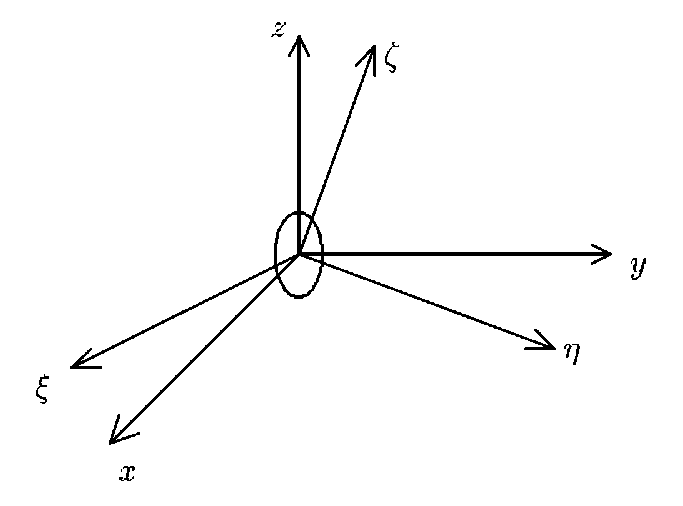
\includegraphics[scale=0.7]{Ris/ris_eps/ris1_01.eps}}}

\risp{1}{Молекулярная и
пространственная системы координат} 
\end{figure}

В дальнейшем будем обозначать координаты пространственной системы
буквами $x,y,z$ (индексы $i,k$ и т.~д.), координаты молекулярной
системы~--- буквами $\xi,\eta,\zeta$ (индексы $\sigma,\tau$ и
т.~д.) или цифрами 1, 2, 3. Удобнее всего выражать направляющие
косинусы $(\sigma i)$ через углы Эйлера $\varphi,\psi,\vartheta$
(рис. 1.2).\vskip -2mm

\begin{figure}[tbp]
\centerline{\hbox{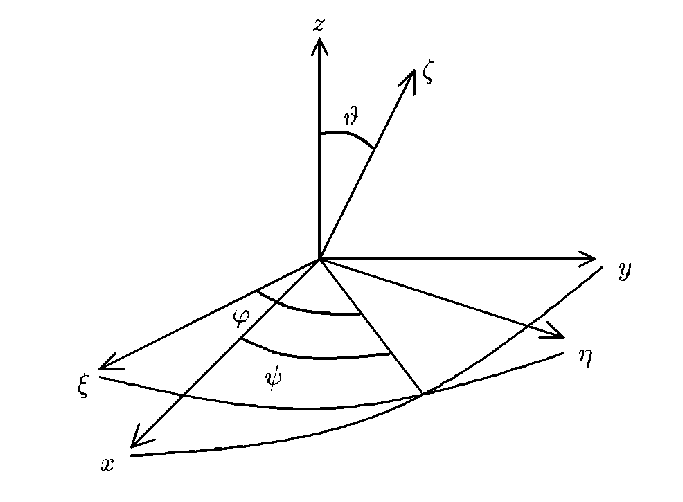
\includegraphics[scale=0.75]{Ris/ris_eps/ris1_02.eps}}}

\risp{2}{Углы Эйлера}
\end{figure}
 
Имеем таблицу значений направляющих косинусов (табл. 1.1). 

\tabp{1}{} 

\centerline{\hbox{\includegraphics[scale=1]{Ris/ris_eps/tab1_01.eps}}}

Во всех задачах мы столкнемся с необходимостью
усреднения различных выражений, содержащих направляющие косинусы,
по всевозможным расположениям системы $\sigma$ относительно
системы $i$. Считая эти расположения равновесными, имеем:
$$f\left\{(\sigma i),(\tau k),\hbox{...}\right\}=
{\int\limits_{0}^{2\pi}\int\limits_{0}^{2\pi}\int\limits_{0}^{\pi}
fd\varphi d\psi \sin\vartheta d\vartheta\over
\int\limits_{0}^{2\pi}\int\limits_{0}^{2\pi}\int\limits_{0}^{\pi}
d\varphi d\psi \sin\vartheta d\vartheta}=$$ $$={1\over 8\pi^2}
\int\limits_{0}^{2\pi}\int\limits_{0}^{2\pi}\int\limits_{0}^{\pi}
fd\varphi d\psi \sin\vartheta d\vartheta.\noq$$ Нам придется иметь
дело с функциями $f$ от направляющих косинусов в первой, второй,
третьей и четвертой степени. Легко видеть, что
$$\overline{(\sigma i)}=\overline{(\zeta
z)}=\overline{\cos\vartheta}=0,\noq$$ так же сразу находим
$$\overline{(\sigma i)^2}=\overline{(\zeta
z)^2}=\overline{\cos^2\vartheta}={1\over3}$$ и
$$\overline{(\sigma i)(\sigma j)}=\overline{(\sigma i)(\tau
j)}=\overline{(\sigma i)(\tau i)}=0,$$ или
$$\overline{(\sigma i)(\tau
j)}={1\over3}\delta_{\sigma\tau}\delta_{ij}. \noq$$ Из функций
третьего порядка отличны от нуля только произведения направляющих
косинусов, не содержащие повторяющихся индексов:
$$\overline{(\xi x)(\eta y)(\zeta z)}=
\overline{(\eta x)(\zeta y)(\xi z)}=\overline{(\zeta x)(\xi
y)(\eta z)}=$$$$= -\overline{(\xi x)(\eta y)(\zeta
z)}=-\overline{(\eta x)(\xi y)(\zeta z)}= -\overline{(\zeta
x)(\eta y)(\xi z)}={1\over6}.\noq$$ Функции четвертого порядка,
отличные от нуля:
\begin{plain}$$\eqalign{
&\overline{(\sigma i)^4}={1\over5},\cr &\overline{(\sigma
i)^2(\tau i)^2}=\overline{(\sigma i)^2(\sigma j)^2}={1\over15},\cr
&\overline{(\sigma i)^2(\tau j)^2}={2\over15},\cr
&\overline{(\sigma i)(\sigma j)(\tau i)(\tau j)}={1\over30},\cr
&\sigma\not=\tau,\hskip 4mm i\not=j. }\noq$$\end{plain} Все эти результаты
могут быть получены непосредственным интегрированием \eqn{38}, с
учетом эквивалентности всех трех осей в каждой системе координат.

\subzag{Симметрия молекул и тензор поляризуемости} 
Молекулы обладают определенной симметрией расположения атомов.
Зная симметрию молекулы, мы можем сделать ряд выводов о ее
электрических и оптических свойствах. Хотя физические свойства
молекулы определяются в основном строением электронных оболочек
атомов, из которых она состоит, однако, свойства симметрии в
расположении электронов и связей обязательно те же, что и в
расположении ядер.

Будем говорить о молекуле как о системе точечных атомов. 
Заменив молекулу системой материальных точек, мы, конечно, 
лишаемся ряда важнейших ее свойств, но сохраняем свойства симметрии, 
которые при таком рассмотрении становятся особенно ясными.

Мы называем операциями симметрии такие перемещения точек в системе, 
которые сохраняют конфигурацию и свойства системы. Такими операциями 
в случае систем, состоящих из конечного числа точек, являются отражения 
и вращения. Система может иметь плоскости симметрии --- такие плоскости, 
отражение в которых не изменяет свойств системы. Например, молекула Н$_{2}$0
 имеет две плоскости симметрии (рис. 1.3) --- плоскость самой молекулы 
и перпендикулярную ей плоскость, проходящую по биссектрисе угла НОН. 
Отражение всех трех атомов в каждой из этих плоскостей, как в зеркале, 
не меняет молекулы. Так, например, отражение атомов H$^{(1)}$, H$^{(2)}$ 
во второй плоскости меняет их местами, отчего сама молекула не изменяется, 
так как оба атома тождественны. Плоскости симметрии обозначаются буквой $\sigma$. 
Второй вид элементов симметрии --- это оси вращения. Мы говорим, что система точек 
имеет ось\  симметрии порядка $n$,  если поворот всей системы вокруг такой оси на 
угол ${360\hbox{°}\over n}$ или ${{360\hbox{°} *2}\over n}, ..., {{360\hbox{°} *(n-1)}\over nC_n}$ 
не меняет свойств системы. Ось симметрии $n$-го порядка обозначается $C_{\hbox{n}}$. 
Так, молекула Н$_2$0, кроме уже рассмотренных плоскостей симметрии, обладает 
осью симметрии второго порядка $C_2$, проходящей по линии пересечения плоскостей --- 
по биссектрисе угла НОН. Поворот связей ОН на 360° : 2 = 180° вокруг 
этой оси переводит одинаковые атомы и связи друг в друга и свойств молекулы не меняет.

\begin{figure}[tbp]
\centerline{\hbox{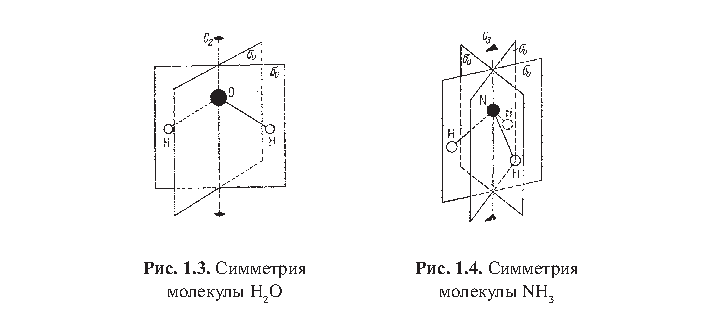
\includegraphics[scale=1]{Ris/ris_eps/ris1_03.eps}}}

\end{figure}
Молекула аммиака NH$_3$ имеет ось третьего порядка $C_3$, проходящую вдоль 
высоты правильной тригональной пирамиды. Операциями симметрии являются повороты 
вокруг этой оси на угол 360° : 3 = 120° и угол 360° $\cdot$ 2~:\linebreak : 3~= 240°. И тот 
и другой повороты не меняют свойств молекулы. Очевидно, что через каждую из связей 
N--Н и ось $C_3$ в молекулу NH$_3$ проходит плоскость симметрии $\sigma_v$; 
значок $v$ указывает, что плоскость вертикальная и в ней лежит ось симметрии (рис. 1.4).

\begin{figure}[tbp]
\centerline{\hbox{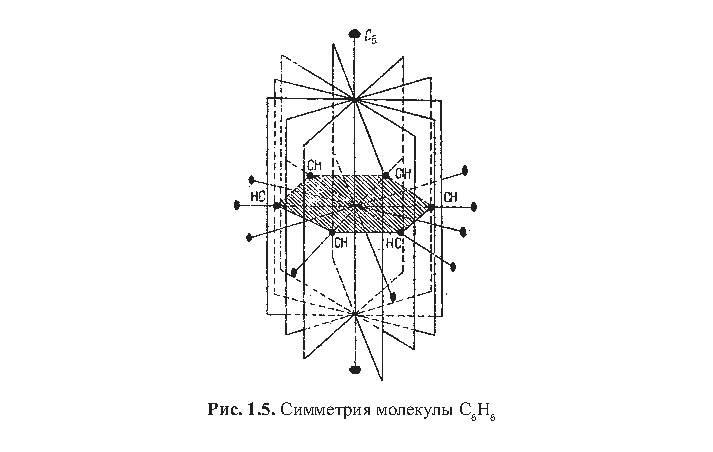
\includegraphics[scale=1]{Ris/ris_eps/ris1_05.eps}}}

\end{figure}

Молекула бензола имеет ось шестого порядка $C_6$, проходящую через центр правильного 
плоского шестиугольника, каким является бензол, перпендикулярно его плоскости. 
Самосовмещение атомов достигается при поворотах этой оси на 360° : 6 = 60°, 360° $\cdot$ 2 : 6 = 120°, 360° $\cdot$ 3 : 6 = 180°, 360° $\cdot$ 4: 6 = 240°, 360° $\cdot$ 5 : 6 = 300°. Сама плоскость бензола обозначается $\sigma_h$; значок $h$ указывает, 
что плоскость симметрии горизонтальная, перпендикулярная оси. Одновременно бензол имеет целый ряд других 
элементов симметрии~--- 6 осей второго порядка, лежащих в плоскости молекулы,- и 6 вертикальных
 плоскостей симметрии, перпендикулярных к $\sigma_h$, а также, как мы увидим, центр симметрии (рис. 1.5).

Порядки осей симметрии, встречающихся в молекулах, --- 2, 3, 4, 5, 6. Кроме того, возможен и порядок бесконечности --- в тех случаях, когда поворот вокруг оси на любой малый или большой угол сохраняет свойства молекулы. Это, очевидно, имеет место только в случае линейных молекул Н$_2$, СO$_2$, HCN, С$_3$O$_2$ и т.~п. Осью бесконечно высокого порядка является сама ось молекулы.

Третий вид элементов симметрии~--- центр симметрии. Центром симметрии системы точек называется точка, отражение в которой всех точек системы не меняет ее свойств. Так, молекула транс-дихлорэтилена имеет центр симметрии, а молекула цис-дихлор-этилена его не имеет. Молекула бензола имеет центр симметрии, NH$_3$ и Н$_2$O его не имеют. Центр симметрии обозначается буквой $i$.


\begin{figure}[tbp]
\centerline{\hbox{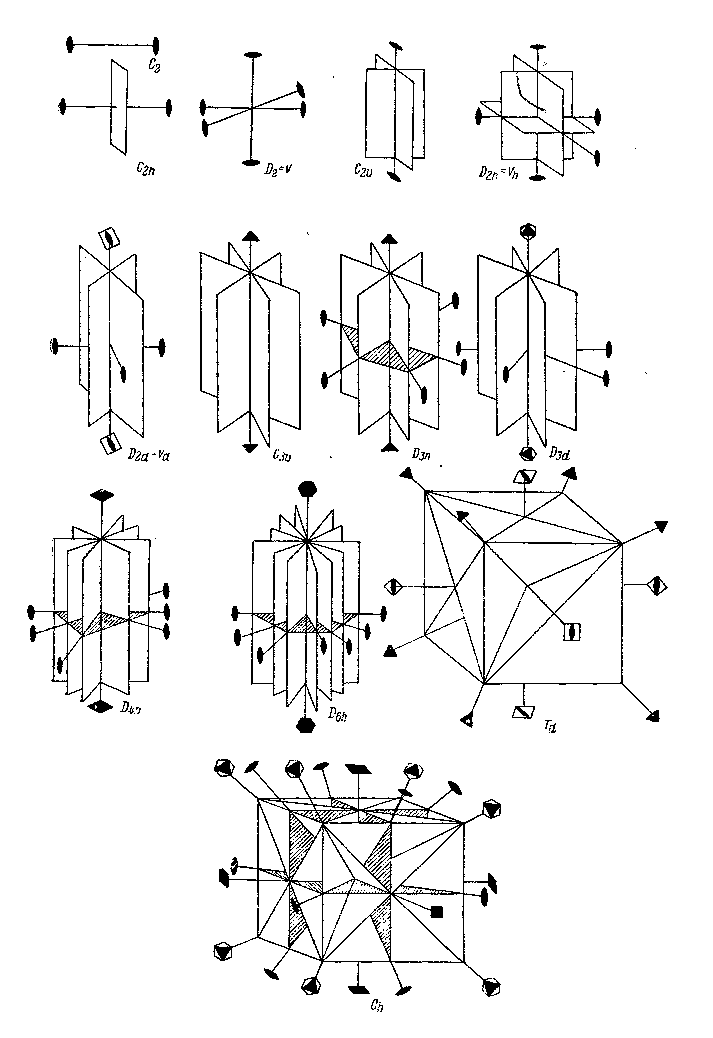
\includegraphics[scale=1]{Ris/ris_eps/ris1_06.eps}}}

\risp{6}{Группы симметрии}
\end{figure}
Наконец, в молекулах возможен еще один вид симметрии, более сложный, сочетающий вращение с отражением. Это --— вращение вокруг оси с последующим отражением в плоскости, перпендикулярной к этой оси. Такие зеркально-поворотные оси обозначаются $S_n$. Так,   молекула   СС1$_4$  имеет  зеркально-поворотные   оси   четвертого порядка   $S_4$. Поворачивая связи \hbox{С--С1} на 360°~:~4 = 90° вокруг вертикальной оси, проходящей по общей биссектрисе двух  тетраэдрических  углов ClCCl, и затем отражая их в плоскости, проходящей через атом С перпендикулярно этой оси, мы получим самосовмещение связей и атомов (рис. 1.6). Легко увидеть, что зеркально-поворотная ось второго порядка эквивалентна центру симметрии, т. е. $S_2\equiv i$.

\begin{figure}[tbp]
\tabp{2}{Группы симметрии}

\centerline{\hbox{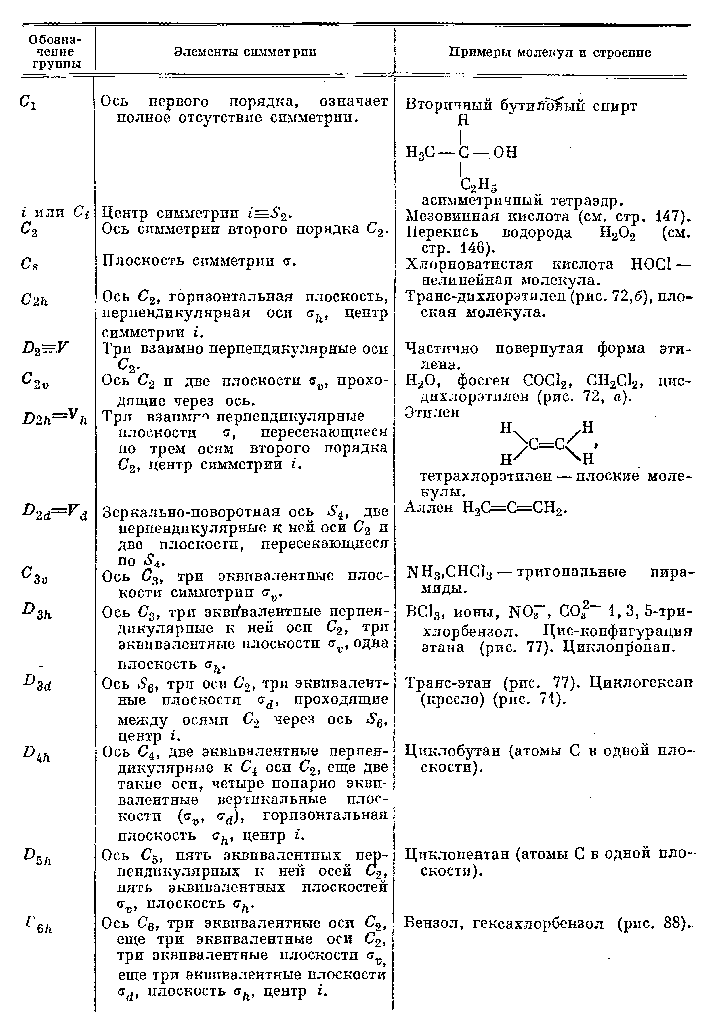
\includegraphics[scale=1]{Ris/ris_eps/tab1_02.eps}}}

\end{figure}

\begin{figure}[tbp]
{\itshape\small\hfill Окончание таблицы 1.2}

\centerline{\hbox{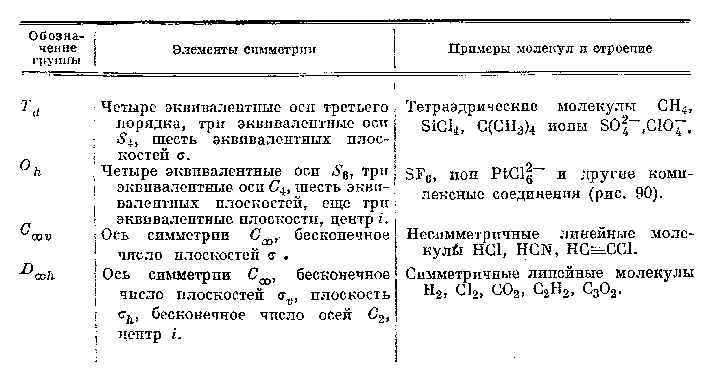
\includegraphics[scale=1]{Ris/ris_eps/tab1_02a.eps}}}


\end{figure}

Сочетание в одной системе нескольких различных элементов симметрии автоматически приводит к появлению новых элементов симметрии. Так, линия пересечения двух взаимно перпендикулярных плоскостей симметрии всегда является осью симметрии молекулы (например, Н$_2$O). Чем больше число различных элементов симметрии, тем выше симметрия молекулы.
Рассмотренные операции симметрии обладают тем свойством, что они оставляют неподвижной по крайней мере одну точку в пространстве. При отражении в центре неподвижным является этот центр, при отражении в плоскости неподвижными являются все точки этой плоскости. При повороте вокруг оси неподвижными остаются все точки этой оси. При сочетании элементов симметрии одна точка обязательно остается неподвижной. Она необязательно совпадает в случае нормальной конфигурации молекулы с одним из атомов. Примером может служить молекула этилена C$_2$H$_4$, для которой при операциях симметрии неподвижным остается центр симметрии, совпадающий с серединой двойной связи C$=$C. Поэтому группы симметрии, представляющие совокупность поворотов и отражений, переводящих нормальную конфигурацию саму в себя, называют точечными группами симметрии.

Рассмотрим возможные группы симметрии молекул. Наиболее важные из них представлены в табл. 1.2, в той же таблице приведены примеры соответствующих молекул. На рисунках, дополняющих табл. 1.2, приведены наглядные изображения групп симметрии.



Теперь рассмотрим связь тензора поляризуемости с симметрией
молекул. Любые физические свойства молекул в значительной степени
определяются их симметрией. Как указывалось ранее, физические
величины, в частности поляризуемость, выражающие свойства
анизотропного тела, имеют характер тензоров. Большинство молекул
являются оптически анизотропными. Это означает, что как величина,
так и направление индуцированного дипольного момента зависят от
ориентации молекулы в электромагнитном поле.

Пусть на произвольно ориентированную молекулу действует поле
$E_x$, которое индуцирует в молекуле дипольный момент $\vec p$,
проекции которого на оси координат пропорциональны $E_x$:
$$p_x=\alpha_{xx}E_x;\hskip 4mm p_y=\alpha_{yx}E_x;\hskip 4mm
p_z=\alpha_{zx}E_x.$$ В общем случае
$$p_i=\sum\limits_k\alpha_{ik}E_k;\hskip 4mm i,k=x,y,z\ ,\noq$$
где $\alpha_{ik}$ --- симметричный тензор второго ранга.

В каждой молекуле имеются молекулярные оси поляризуемости: 1,~2,~3.
То есть если поле направлено вдоль какой-нибудь оси, то
направление $\vec p$ строго параллельно направлению этого поля:
$$\vec p_1=\alpha_1\vec E;\hskip 4mm\vec p_2=\alpha_2\vec
E;\hskip 4mm\vec p_3=\alpha_3\vec E,$$ где
$\alpha_1,\alpha_2,\alpha_3$ --- главные поляризуемости молекулы.
Знание их в молекулярной системе координат позволяет найти
компоненты тензора $\alpha_{ik}$ в любой системе координат.

Напишем формулы преобразования тензора поляризуемости от главных
молекулярных осей 1,2,3 к лабораторной системе координат.
Направление вектора $E$ задано в пространственно неподвижной
системе координат $x,y,z$. Рассмотрим дипольный момент,
индуцированный полем в молекуле, выразив составляющие момента в
молекулярной системе координат 1,~2,~3, совпадающей с системой
главных осей эллипсоида поляризуемости молекулы (см.~рис.~ 1.7).

\begin{figure}[tbp]
\centerline{\hbox{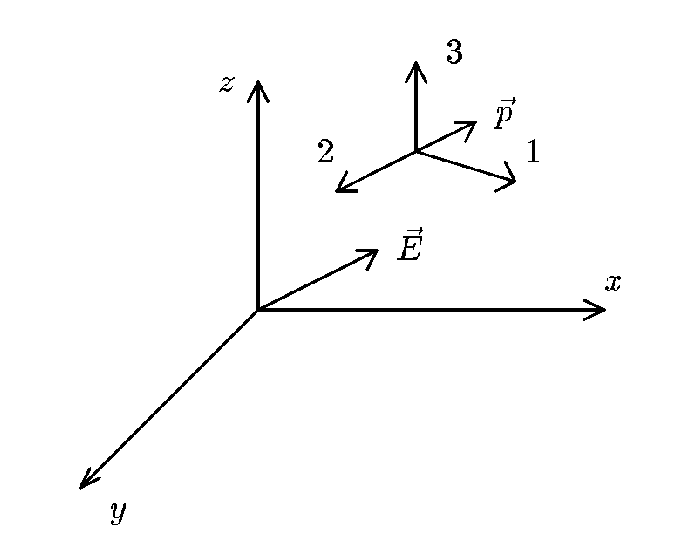
\includegraphics[scale=0.7]{Ris/ris_eps/ris1_07.eps}}}

\risp{7}{Дипольный момент в
молекулярной и пространственной } 
\centerline{системах координат}
\end{figure}
В этой системе имеем:
$$E_{\sigma}=\sum\limits_{i=x,y,z}E_i(\sigma i),\hskip 4mm
\sigma=1,2,3\ ,\noq$$
\begin{plain}$$\eqalign{
p_{\sigma}=&\hbox{\ }\alpha_{\sigma}E_{\sigma}=\alpha_{\sigma}\sum\limits_i
E_i(\sigma i),\cr p_i=&\sum\limits_{\sigma}p_{\sigma}(\sigma i)
.}\noq$$\end{plain} Проекции вектора $\vec p$ на оси 1,~2,~3:
$p_1=\alpha_1E_1,\ p_2=\alpha_2E_2,\ p_3=\alpha_3E_3$, но из
формул \eqn{44-45} следует:
$$p_x=\sum\limits_{\sigma}\alpha_{\sigma}(\sigma
x)^2E_x+\sum\limits_{\sigma}\alpha_{\sigma}(\sigma x)(\sigma
y)Ey+\sum\limits_{\sigma}\alpha_{\sigma}(\sigma x)(\sigma
z)E_z.\noq$$ При сравнении выражения \eqn{46} с формулой \eqn{43},
можно сделать вывод, что они тождественно равны, если множители
при $E_x$ в формулах равны:
\begin{plain}$$\eqalign{
\alpha_{xx}=&\hbox{\ }\alpha_1(1x)^2+\alpha_{2}(2x)^2+\alpha_3(3x)^2,\cr
\alpha_{yy}=&\hbox{\ }\alpha_1(1y)^2+\alpha_{2}(2y)^2+\alpha_3(3y)^2,\cr
\alpha_{zz}=&\hbox{\ }\alpha_1(1z)^2+\alpha_{2}(2z)^2+\alpha_3(3z)^2,\cr
\alpha_{xy}=&\hbox{\ }\alpha_{yx}=\alpha_1(1x)(1y)+\alpha_{2}(2x)(2y)+\alpha_3(3x)(3y),\cr
\alpha_{xz}=&\hbox{\ }\alpha_{zx}=\alpha_1(1x)(1z)+\alpha_{2}(2x)(2z)+\alpha_3(3x)(3z),\cr
\alpha_{yz}=&\hbox{\ }\alpha_{zy}=\alpha_1(1x)(1z)+\alpha_{2}(2y)(2z)+\alpha_3(3y)(3z)
.}\noq$$\end{plain}Формулы \eqn{47} --- формулы преобразования тензора
поляризуемости от главных осей к произвольной системе координат. В
случае если одна из лабораторных осей, например, ось $z$, совпадает
с осью 3, угол между этими осями равен нулю, и тогда:
$$\cos(3z)=1;\hskip 3mm\cos(3x)=\cos(3y)=\cos(1z)=\cos(2z)=0,$$
и
\begin{plain}$$\eqalign{
\alpha_{xx}=&\alpha_1(1x)^2+\alpha_2(2x)^2,\cr
\alpha_{yy}=&\alpha_1(1y)^2+\alpha_2(2y)^2;\hskip
4mm\alpha_{zz}=\alpha_2,\cr
\alpha_{xy}=&\alpha_1(1x)(1y)+\alpha_2(2x)(2y);\hskip 4mm
\alpha_{xz}=\alpha_{yz}=0. }$$\end{plain} 

Таким образом, если ось $z$
является осью тензора поляризуемости, то компоненты тензора
$\alpha_{xz}$ и $\alpha_{yz}$ равны нулю. И соответственно, если
ось $y$ --- главная ось тензора, то $\alpha_{xy}=\alpha_{zy}=0$;
если ось $x$: $\alpha_{xy}=\alpha_{xz}=0$.

Направление главных осей поляризуемости молекул определяется
структурой молекул и их симметрией. Симметричный тензор второго
ранга, каким является тензор поляризуемости, обладает центром
симметрии независимо от того, обладает ли сама молекула таким
центром. Иными словами, значение тензора не меняется при замене
всех координат их отрицательными значениями. В самом деле,
перейдем от тензора $\alpha_{ik}$, записанного в системе координат
$x,y,z$, к тензору $\alpha'_{ik}$, записанному в системе координат
$x'=-x,\ y'=-y,\ z'=-z$. При преобразовании системы координат
тензор второго ранга трансформируется, как произведение двух
векторов, и углы между молекулярными и лабораторными осями
изменятся: $\angle(1'x)=\pi-\angle(1x); \
\angle(1'y)=\pi-\angle(1y)$, следовательно: $\cos(1'x)=-\cos(1x);\
\cos(1'y)=-\cos(1y)$ и так далее. Так как в формулы преобразования
тензора поляризуемости \eqn{47} косинусы входят как квадраты или
произведения, то можно сделать вывод, что при отражении в центре
молекулы компоненты тензора поляризуемости остаются такими же, как
и до отражения: $\alpha'_{xx}=\alpha_{xx};\
\alpha'_{yy}=\alpha_{yy};\ \alpha'_{zz}=\alpha_{zz};
\alpha'_{xy}=\alpha_{xy}$ и т.~д.

Отсюда следует, что любое физическое свойство, представляемое
симметричным тензором второго ранга, есть свойство
центросимметрическое, и, следовательно, в отношении этого свойства
нет разницы между теми классами симметрии, которые обладают или не
обладают центром симметрии. Тензор поляризуемости имеет всего пять
различных форм, соответствующих определенным классам симметрии.

К первому классу относятся молекулы, не имеющие никаких элементов
симметрии или имеющие только центр симметрии: $C_i$, тензор имеет
вид:
$$\left(\matrix{
\alpha_{11}&\alpha_{12}&\alpha_{13}\cr
\alpha_{12}&\alpha_{22}&\alpha_{23}\cr
\alpha_{13}&\alpha_{23}&\alpha_{33}\cr }\right).$$

Второй класс образуют молекулы, принадлежащие к группам симметрии
$C_s,\ C_2,\ C_{2h}$. Группа $C_s$ имеет только плоскость
симметрии. Проводим оси $x,y$ в плоскости симметрии, а ось $z$
--- перпендикулярно к ней. Направления 1,~2,~3 нам заранее
неизвестны. Отразим молекулу в плоскости симметрии $(xy)$. Тогда
все координаты $z$ у атомов молекулы меняют знак, а координаты $x$
и $y$ остаются неизменными. Оси 1,~2,~3 меняют направление на
\hbox{$1'$, $2'$, $3'$}. Углы между осью $z$ и 1,~2,~3 и осью $z$ и \hbox{$1'$, $2'$, $3'$}
связаны условиями: $\angle(1'z)=\pi-\angle(1z); \
\angle(2'z)=\pi-\angle(2z); \ \angle(3'z)=\pi-\angle(3z),$ откуда
следует, что $\cos(1'z)=-\cos(1z);\ \cos(2'z)=-\cos(2z) \
\cos(3'z)=$\linebreak$=-\cos(3z).$ Так как отражение в плоскости является
преобразованием симметрии, то все компоненты тензора
поляризуемости должны оставаться неизменными, т.~е.
$\alpha'_{ik}=\alpha_{ik}$, в том числе:
$\alpha'_{xz}=\alpha_{xz};$\linebreak$\alpha'_{yz}=\alpha_{yz}$. Но
подставив в формулы преобразования соответствующие вышеуказанные
углы, получим: $\alpha'_{xz}=-\alpha_{xz};\
\alpha'_{yz}=-\alpha_{yz}$. Противоречие будет устранено, если
$\alpha_{xz}=\alpha_{yz}=0$. То есть если молекула имеет
плоскость симметрии, то нормаль к ней является главной осью
тензора поляризуемости. Направления двух других осей неизвестны,
они лежат в плоскости симметрии.

Для группы $C_2$: если в молекуле имеется ось симметрии $C_2$, то
она совпадает с одной из главных осей тензора поляризуемости.
Доказательство~то~же.

Молекулы группы $C_{2h}$ имеют ось симметрии $C_2$ и плоскость,
перпендикулярную к ней. Когда ось  и нормаль к плоскости
совпадают, то все сводится к случаям групп симметрии $C_2$ и
$C_s$. Тензор во всех трех случаях будет иметь вид:
$$\left(\matrix{
\alpha_{11}&\alpha_{12}&0\cr \alpha_{12}&\alpha_{22}&0\cr
0&0&\alpha_{33}\cr }\right).$$

Третий класс образуют молекулы групп симметрии $C_{2v},\ D_2,\
D_{2h}$. Тензор поляризуемости имеет центр симметрии, три взаимно
перпендикулярных оси второго порядка и плоскости симметрии,
проходящие через любые две оси. Направление осей 1,~2,~3
соответствует направлениям трех осей $C_2$.\linebreak Тензор имеет вид:
$$\left(\matrix{
\alpha_{11}&0&0\cr 0&\alpha_{22}&0\cr 0&0&\alpha_{33}\cr
}\right).$$

К четвертому классу принадлежат все молекулы, имеющие ось
симметрии высшего порядка: $C_3,\ C_4$ и более высокого порядка,
включая $C_{\infty}$. Тензор вырождается в аксиально-симметричный
с двумя главными значениями~$\alpha$: вдоль оси высшего порядка
--- $\alpha_{\parallel}$, и перпендикулярно оси ---
$\alpha_{\perp}$ (группы симметрии $S_4,\ D_{2h}$). Покажем это на
примере оси четвертого порядка. Проведем координатные оси $x,y,z$
и 1,~2,~3. Направим ось $z$ по направлению, совпадающему с
направлением оси $C_4$. Являясь одновременно и осью второго
порядка, она является главной осью тензора поляризуемости. Пусть
это будет ось 3. Компоненты $\alpha_{xz}$ и $\alpha_{yz}$ равны
нулю. Повернем молекулу вокруг оси~$z$ на $90^{\circ}$: $x'=y;\
y'=-x;\ z'=z$. Вместо поворота молекулы вместе с осями 1,~2 можно
повернуть оси $x,y$ вокруг $z$. Тогда: $\angle(1x')=\angle(1y);\
\angle(2x')=$\linebreak$=\angle(2y);\ \angle(1y')=\pi-\angle(1x);\
\angle(2y')=\pi-\angle(2x)$. Следовательно: $\cos(1x')=$\linebreak$=cos(1y);\
\cos(2x')=\cos(2y);\ \cos(1y')=-\cos(1x);\ \cos(2y')=-\cos(2x)$.
После поворота компонента получаем:
$\alpha'_{xy}=\alpha_1(1x')(1y')+\alpha_{2}(2x')(2y')+$\linebreak$+\alpha_{3}(3x')(3y')$.
Можно показать, что $\alpha_{xy}=0$. Действительно, ранее мы
показали, что в подобном случае $\cos(3x')=\cos(3y')=0$. Заменяя
$(1x')$ на $(1y)$ и $(1y')$ на $-(1x)$; $(2x')$ на $(2y)$ и
$(2y')$ на $-(2x)$, находим
$\alpha'_{xy}=$\linebreak$=-\alpha_1(1y)(1x)-\alpha_2(2y)(2x)=-\alpha_{xy}$. Но
поворот на $90^{\circ}$ вокруг своей оси является операцией
симметрии, и, следовательно, $\alpha'_{xy}=-\alpha_{xy}=0$. Значит
оси $x$ и $y$ являются главными осями тензора, независимо от их
ориентации в плоскости, перпендикулярной оси симметрии $C_4$:
$\alpha_1=\alpha_2=\alpha_{\perp},\ \alpha_3=\alpha_{\parallel}$.

Таким образом, тензор имеет вид:
$$\left(\matrix{
\alpha_{11}&0&0\cr 0&\alpha_{22}&0\cr 0&0&\alpha_{33}\cr
}\right),$$ где направление 3 совпадает с $C_{\infty}$.

Есть молекулы, имеющие несколько осей высшего порядка, пересекающихся в
одной точке, и бесконечное множество плоскостей симметрии,
проходящих через эту точку. Сама эта точка является центром
симметрии. Это молекулы кубической симметрии $K_h$. Вид тензора:
$$\left(\matrix{
\alpha_{11}&0&0\cr 0&\alpha_{11}&0\cr 0&0&\alpha_{11}\cr
}\right).$$

\vskip 5 mm
\noindent{\bfseries Литература:}
\vskip 2 mm
1. {\itshape Волькенштейн М. В.} Молекулярная оптика. --- Гостехиздат, 1944.

2. {\itshape Тамм И. Е.} Основы теории электричества. --- Гостехиздат, 1949.

3. {\itshape Волькенштейн М. В.} Строение и физические свойства молекул.~--- Москва--Ленинград, АН СССР, 1955.

4. {\itshape  Вукс М. Ф.}
Электрические и оптические свойства молекул и конденсированных сред.~--- Л.: Издательство ЛГУ, 1984.

5. {\itshape Волькенштейн М. В., Еляшевич М. А., Степанов Б. И.}
Колебания молекул, том I.~--- М., 1949.

6. {\itshape Борн М.}
Оптика. --- ОНТИУ, 1937.\thispagestyle{empty}
